\section{Fonctionnement}\label{sec:works}

\acrshort{tor} est un réseau de serveurs, appelés nœuds ou relais, permettant aux utilisateurs d'accéder à Internet de manière anonyme.
Son fonctionnement est basé sur le principe de la transmission de données en couches chiffrées, d'où son nom qui fait référence à l'oignon ainsi qu'à ses couches. 
Cette section détaillera les étapes clés du processus permettant l'utilisation de \acrshort{tor} de l'"\nameref{subsec:initialisation}" à l' "\nameref{subsec:utilisation}" en passant par la "\nameref{subsec:construction}".

\subsection{Initialisation}\label{subsec:initialisation}

L'utilisateur initie la connexion avec le premier noeud.
\begin{enumerate}
  \item \textbf{Démarrage du Proxy Oignon (\acrshort{op}):} Il exécute d'un proxy oignon (\acrshort{op} \textit{Onion Proxy}) qui sert d'interface entre l'application utilisateur et le réseau \acrshort{tor}. 
  \item \textbf{Récupération des répertoires:} L'\acrshort{op} récupère la liste des  \acrshort{or}  actifs depuis les serveurs d'annuaires ainsi que les adresses, clés publiques et politiques de sorties.
  Ces informations signées permettent de vérifier leur authenticité.
  \item \textbf{Sélection des noeuds:}
  Les n\oe uds du circuit sont sélectionnés sur base de critères géographiques et liés aux politiques de sortie. De cette manière, l'anonymat ainsi que la compatibilité avec les besoins utilisateurs sont garantis.
  \item \textbf{Initialisation TLS:} L'\acrshort{op} établit une connexion \acrshort{tls} avec le gardien d'entrée (\textit{entry node}) afin de garantir la confidentialité et l'intégrité des communications initiales.
  Ce nœud connaît l'origine de la connexion mais ne connaît pas la destination finale des données.
\end{enumerate}

\subsection{Construction}\label{subsec:construction}

\acrshort{tor} crée un circuit chiffré à travers le réseau. 
\begin{enumerate}
  \item \textbf{Négociation Clé \acrlong{dh}:} Pour chaque  \acrshort{or}  sur le circuit, l'\acrshort{op} envoie une cellule "CREATE" contenant la première moitié d'un échange de clés \acrshort{dh}, chiffrée avec la clé publique de l' \acrshort{or}  (clé d'oignon). 
  Ce processus établit une clé de session symétrique partagée qui garantit que seul l' \acrshort{or}  peut déchiffrer et ainsi répondre à la requête.
  \item  \textbf{Extension du circuit:} L'\acrshort{op} envoie des cellules "RELAY EXTEND" à travers le circuit existant vers les autres  \acrshort{or}  pour négocier les nouvelles clés de session symétriques via \acrshort{dh}.
  Chaque  \acrshort{or}  ajoute sa propre couche de chiffrement afin de s'assurer que seuls les noeuds suivants puisse lire les instructions pour l'extension du circuit.
  \item \textbf{Vérification du circuit:} Le chiffrement itératif à chaque étape du circuit assure que chaque  \acrshort{or}  ne puisse accéder qu'aux informations de son prédécesseur et successeur direct.
\end{enumerate}

\subsection{Utilisation}\label{subsec:utilisation}

Les données passent ensuite par plusieurs nœuds intermédiaires (\textit{middle nodes}), où chaque nœud ne connaît que le nœud précédent et le suivant, mais jamais l'ensemble du circuit, comme expliqué dans.
\begin{enumerate}
  \item \textbf{Chiffrement en Couches :} Les données sont encapsulées dans des couches de chiffrement, une pour chaque nœud que le paquet de données traversera.
  \item \textbf{Déchiffrement Progressif :} À chaque étape du circuit, un nœud enlève une couche de chiffrement pour découvrir à quel nœud envoyer le paquet suivant.
  \item \textbf{Destination Finale :} 
  Lorsque les données atteignent le nœud de sortie (\textit{exit node}), la dernière couche de chiffrement est retirée et les données sont envoyées à leur destination finale.
\end{enumerate}

Grâce à ce mécanisme, l'adresse IP de l'utilisateur est masquée, et les données transmises sont rendues indéchiffrables pour les observateurs extérieurs.
Cela assure l'anonymat de l'utilisateur et la confidentialité des informations échangées.


% \subsection{Rôles}

% L'anonymisation implique différents rôles pour les noeuds selectionnés pour créer le circuit.


% \subsubsection{Sélection des Relais}
% Les relais sont choisis selon des critères stricts, visant à optimiser la performance et la sécurité. 
% La sélection tient compte de la bande passante, de la stabilité et de la réputation des relais, minimisant le risque d'attaques malveillantes.


% \subsection{Workflow}

% \begin{figure}[h!]
%   \centering
%   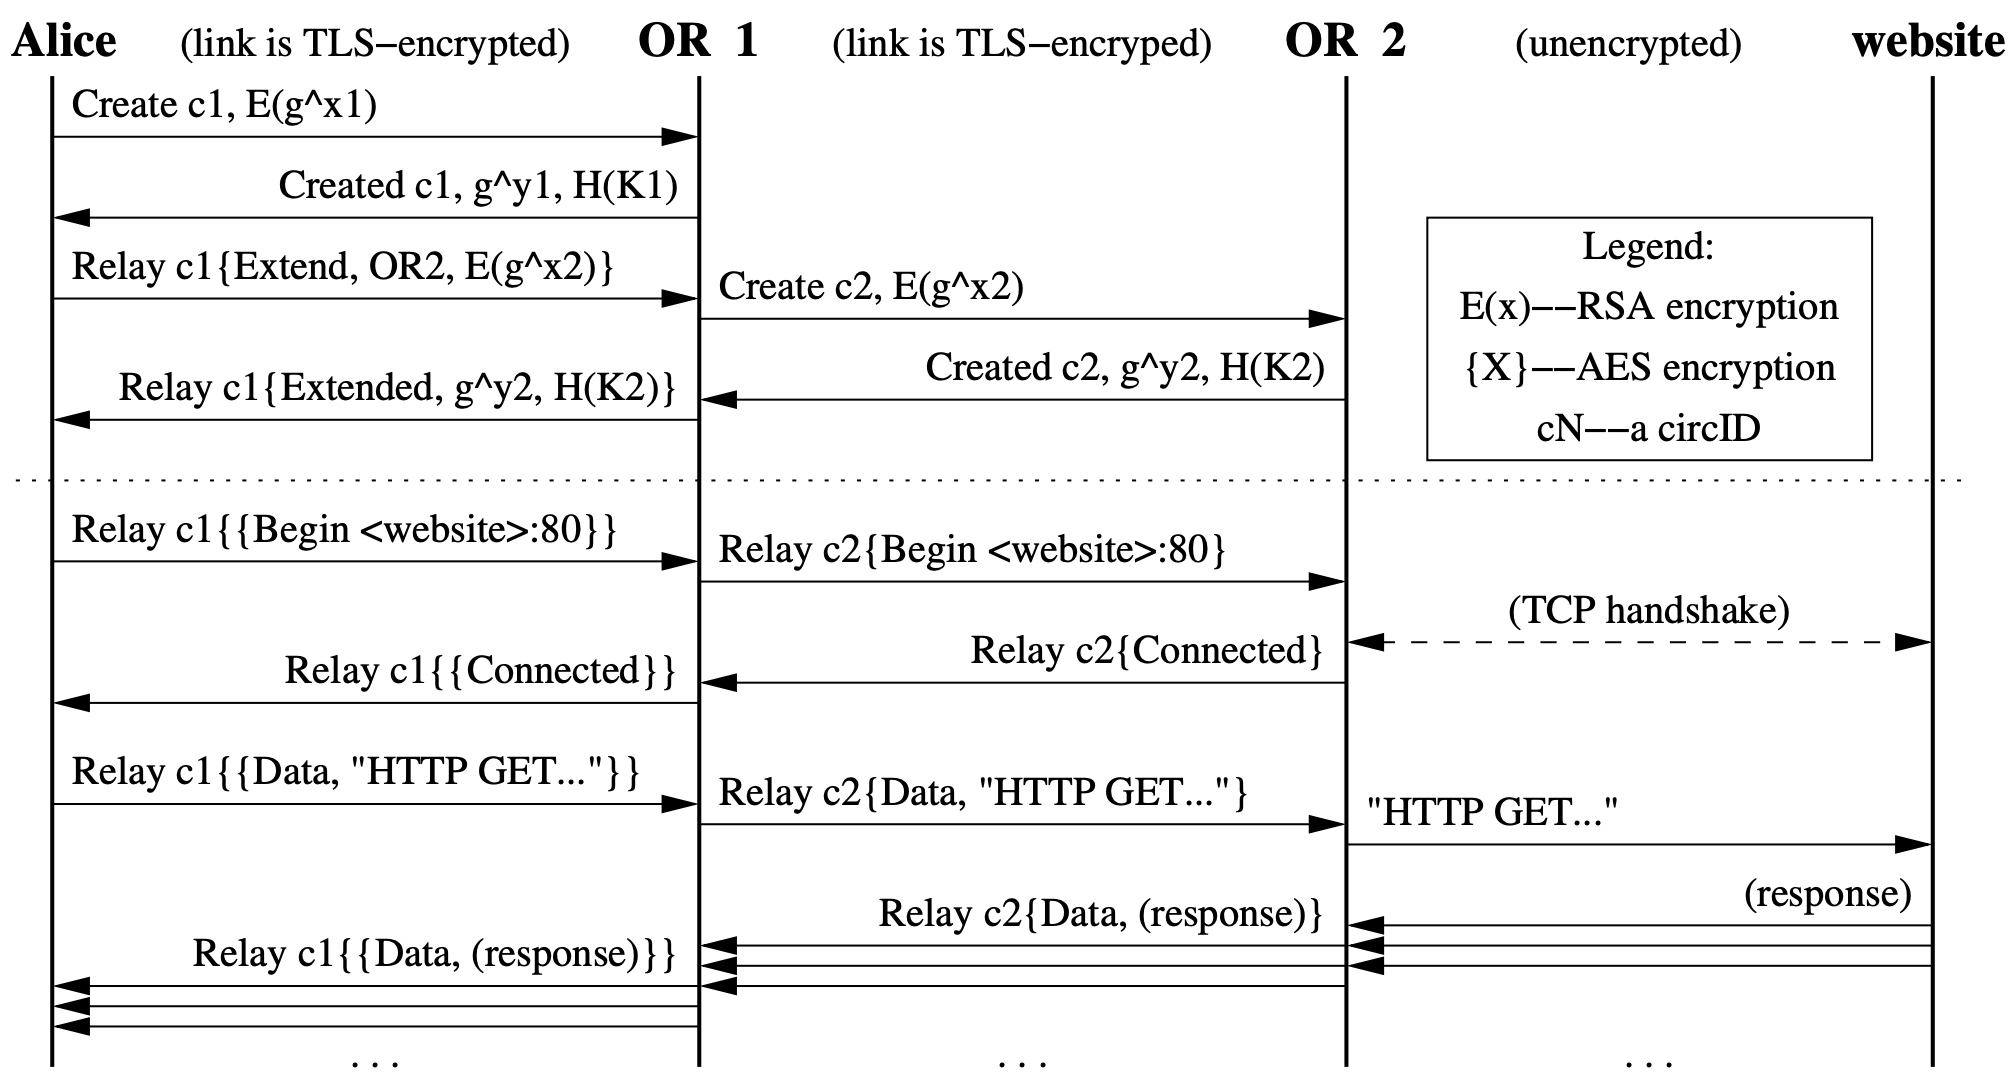
\includegraphics[width=\linewidth]{Images/Diagrams/flow.png}
%   \caption{Circuit à deux Routeurs Onions permettant à Alice de joindre un site web.\cite[Tor: The Second-Generation Onion Router]{dingledine_tor_2004}}
%   \label{fig:flowdiagram}
% \end{figure}

% \subsection{Services cachés}
